%======================================================================
%  AutoDD -- ICDM 2026 poster
%  Board size: 33.1 in x 46.8 in  (841 mm x 1189 mm = A0 portrait)
%  Build:  pdflatex poster.tex   (run twice)
%======================================================================
\documentclass[final]{beamer}
\usepackage[orientation=portrait,size=a0,scale=1.23]{beamerposter}
\usetheme{default}
\usecolortheme{default}
\beamertemplatenavigationsymbolsempty

\usepackage[T1]{fontenc}
\usepackage{lmodern}
\usepackage{amsmath,amssymb}
\usepackage{booktabs}
\usepackage{graphicx}
\usepackage{tikz}
\usepackage{qrcode}
\usepackage{xcolor}
\graphicspath{{assets/}{../images/}}

%---------------------------------------------------------------- palette
\definecolor{icdmblue}{HTML}{0B5FD8}   % logo blue
\definecolor{darkblue}{HTML}{0A2A5E}   % headings
\definecolor{rule}{HTML}{9AA4B2}       % hairlines
\definecolor{panel}{HTML}{F2F5FA}      % block background
\definecolor{accent}{HTML}{C2410C}     % highlight numbers

%---------------------------------------------------------------- paper metadata
\newcommand{\paperid}{DM1326}
\newlength{\hdrH}\setlength{\hdrH}{6.4cm}
\newcommand{\paperurl}{https://github.com/TechyNilesh/AutoDD}

%---------------------------------------------------------------- block style
\setbeamercolor{block title}{fg=white,bg=darkblue}
\setbeamercolor{block body}{fg=black,bg=panel}
\setbeamerfont{block title}{size=\large,series=\bfseries}
\newlength{\blockpad}\setlength{\blockpad}{1.6cm}
\setbeamertemplate{block begin}{
  \vskip8pt
  \begin{beamercolorbox}[wd=\textwidth,colsep*=0ex,ht=3.1ex,dp=1.6ex]{block title}
    \hspace*{\blockpad}\usebeamerfont{block title}\insertblocktitle
  \end{beamercolorbox}
  \begin{beamercolorbox}[wd=\textwidth,colsep*=0ex,vmode]{block body}
  \vskip10pt
  \hspace*{\blockpad}%
  \begin{minipage}{\dimexpr\textwidth-2\blockpad\relax}
}
\setbeamertemplate{block end}{
  \end{minipage}\hspace*{\blockpad}%
  \vskip12pt
  \end{beamercolorbox}\vskip4pt}
\setlength{\leftmargini}{1.8em}
\setlength{\labelsep}{0.6em}
\setbeamertemplate{itemize item}{\color{icdmblue}$\blacktriangleright$}
\setbeamertemplate{itemize subitem}{\color{icdmblue}\textbf{--}}

%---------------------------------------------------------------- outer frame + paper id
\newcommand{\paperidstamp}{%
  \begin{tikzpicture}[remember picture,overlay]
    \node[anchor=south east,font=\bfseries\Large,text=darkblue]
      at ([shift={(-2.6cm,1.4cm)}]current page.south east) {\paperid};
  \end{tikzpicture}}

\begin{document}
\begin{frame}[t]
\vspace*{1.2cm}

%================================================================= HEADER
\raisebox{-0.5\height}{
\includegraphics[height=\hdrH]{icdm_logo.png}}
\hfill
\begin{minipage}[c]{0.645\textwidth}
  \centering
  {\huge\bfseries\color{darkblue}\baselineskip=1.15\baselineskip
   AutoDD: Learning to Select Drift Detectors\\[8pt]
   for Evolving Data Streams\par}
  \vskip16pt
  {\Large Nilesh Verma\textsuperscript{1} \quad Albert Bifet\textsuperscript{1,2} \quad
          Bernhard Pfahringer\textsuperscript{1} \quad Maroua Bahri\textsuperscript{3}\par}
  \vskip8pt
  {\large \textsuperscript{1}AI Institute, University of Waikato, New Zealand \quad
          \textsuperscript{2}T\'el\'ecom Paris, IP Paris, France\\[4pt]
          \textsuperscript{3}CNRS, LIP6, Sorbonne Universit\'e, France\par}
\end{minipage}
\hfill
\begin{minipage}[c]{\dimexpr\hdrH+1.5cm\relax}
  \centering
  \qrcode[height=\hdrH]{\paperurl}\\[6pt]
  {\normalsize\bfseries Code \& Paper}
\end{minipage}

\vskip14pt
{\color{rule}\rule{\textwidth}{2pt}}
\vskip18pt

%================================================================= BODY
\begin{block}{Automated Drift Detector Framework}
{\centering
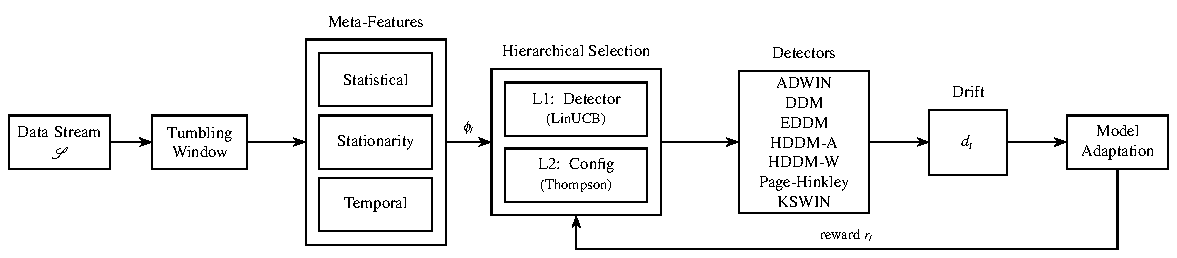
\includegraphics[width=0.92\textwidth]{framework/framework_tikz.pdf}\par}
\vskip10pt
Overview of AutoDD. Meta-features extracted from a tumbling window form the
context $\boldsymbol{\phi}_t$. LinUCB selects a detector, Thompson Sampling
selects its configuration, and the resulting drift signal triggers adaptation.
The reward $r_t$ is then used to update both selection levels.
\end{block}

\begin{columns}[t]

%------------------------------------------------ COLUMN 1
\begin{column}{0.485\textwidth}

\begin{block}{Introduction}
{\centering
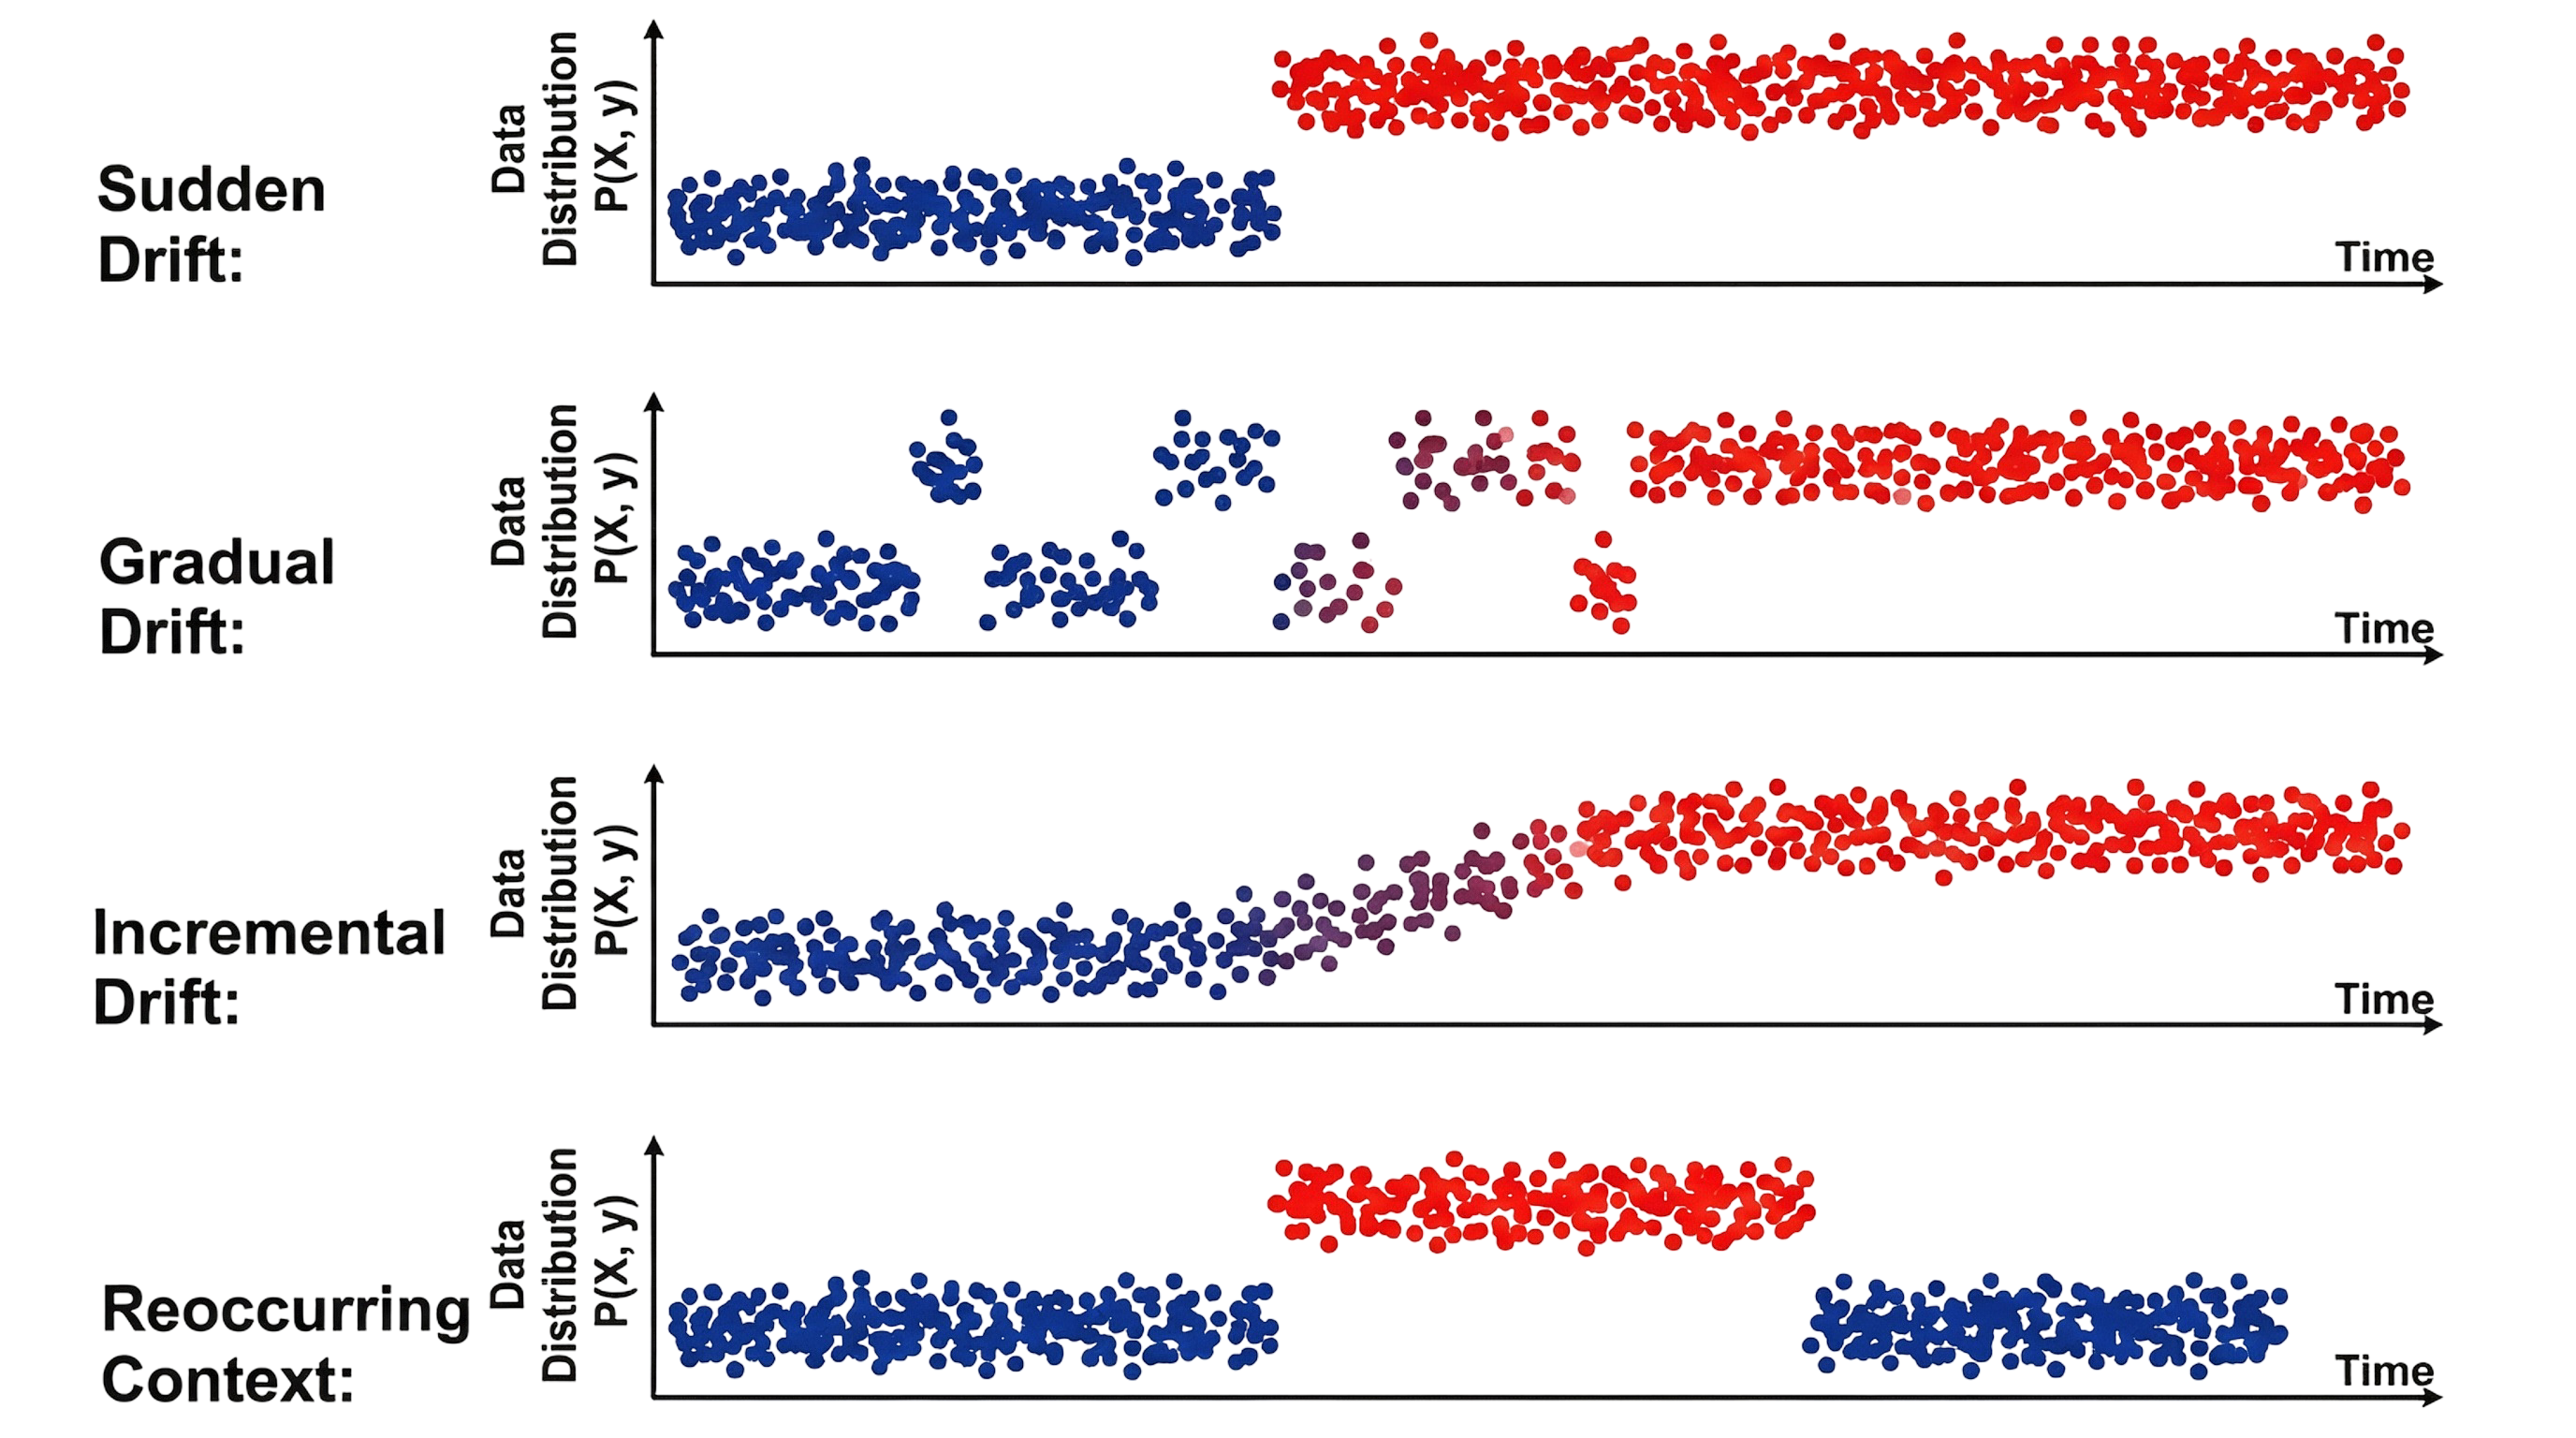
\includegraphics[width=0.76\textwidth]{concept/type_of_drift_detection.png}\\[4pt]
{\small Sudden, gradual, incremental, and recurring drift.}\par}
\vskip12pt
No single drift detector wins everywhere. Each one embeds an assumption about
\emph{how} drift arrives, so a detector tuned for abrupt change reacts slowly to
gradual change, and the right choice shifts as the stream itself evolves.
\vskip10pt
Streaming AutoML automates the \emph{learner}, but pins the \emph{detector} to a
fixed, hand-chosen setting, which leaves a gap in the automation loop.
\vskip10pt
Automating the choice online is hard because
\begin{itemize}
  \item drift labels never arrive, so detector quality must be inferred from a
        \textbf{proxy reward} built from downstream model behaviour, and
  \item the joint space of detectors $\times$ configurations is far too large to
        search as one flat action set.
\end{itemize}
\end{block}

\begin{block}{Problem Formulation}
Given a portfolio $\mathcal{D}=\{D_1,\dots,D_K\}$ where detector $D_i$ has
configuration space $\mathcal{H}_i$, AutoDD selects \emph{jointly} and \emph{online}
\vskip6pt
\begin{equation*}
(D^*_t,\boldsymbol{\eta}^*_t)=\arg\max_{D_i\in\mathcal{D},\,\boldsymbol{\eta}\in\mathcal{H}_i}
\mathbb{E}\!\left[\mathrm{Perf}\big(D_i(\boldsymbol{\eta}),\mathcal{S}_t\big)\mid\boldsymbol{\phi}_t\right]
\end{equation*}
\vskip6pt
with $\boldsymbol{\phi}_t$ the online stream context and $\mathrm{Perf}(\cdot)$ the
downstream model performance.
\end{block}

\begin{block}{Contributions}
\begin{itemize}
  \item \textbf{AutoDD}, the first framework to bring the drift detector itself
        into the automation loop, compatible with any model or AutoML pipeline.
  \item A \textbf{two-level hierarchical bandit} in which LinUCB over online
        meta-features chooses the detector and Thompson Sampling chooses its
        configuration.
  \item Proxy-regret analysis of both levels, plus an evaluation over
        \textbf{ten benchmarks} and two base learners where AutoDD takes the
        best average rank at competitive cost.
\end{itemize}
\end{block}


\begin{block}{AutoDD Method}
\textbf{Context.} 15 online meta-features are computed over a tumbling window and
normalised to $[0,1]$. They cover \emph{statistical} properties (velocity,
dimensionality, sparsity, noise, imbalance), \emph{stationarity} (error
volatility, KL divergence, autocorrelation, mean and variance shift), and
\emph{temporal} structure (trend, periodicity, change frequency and magnitude,
recurrence).
\vskip10pt
\textbf{Level 1, detector selection.} Disjoint-arm LinUCB over $K=7$ detectors
\begin{equation*}
i_t=\arg\max_i\ \boldsymbol{\phi}_t^\top\hat{\boldsymbol{\theta}}_i
+\alpha_{\text{ucb}}\sqrt{\boldsymbol{\phi}_t^\top\mathbf{A}_i^{-1}\boldsymbol{\phi}_t}
\end{equation*}
\textbf{Level 2, configuration selection.} Beta and Bernoulli Thompson Sampling
over $C=5$ configurations per detector.
\vskip10pt
\textbf{Reward without labels.} A bounded proxy $r_t\in[-1,1]$ built from the
windowed accuracy drop $\Delta a_t$, credited only when the change clears the
significance threshold $\tau_{\text{sig}}=0.05$, so noise-driven dips cannot
reinforce spurious detections.
\end{block}


\end{column}

%------------------------------------------------ COLUMN 2
\begin{column}{0.485\textwidth}

\begin{block}{Theory}
\begin{itemize}
  \item \textbf{Level 1.} $R_1(T)=\tilde{O}(m\sqrt{KT})$ for LinUCB under bounded
        features, linear reward, and sub-Gaussian noise.
  \item \textbf{Level 2.} $R_2(T)=\sum_i O(\sqrt{C\,N_i(T)\log N_i(T)})$ for
        Thompson Sampling.
\end{itemize}
\vskip6pt
Both bound \emph{idealised} sub-problems against the proxy objective, so they
are surrogate analyses, not guarantees for the deployed system.
\end{block}

\begin{block}{Results}
Mean over the 5 synthetic and 5 real-world benchmarks, against 12 baselines.
\vskip10pt
{\centering
\begin{tabular}{lcccc}
\toprule
& \multicolumn{2}{c}{\textbf{GaussianNB}} & \multicolumn{2}{c}{\textbf{HAT}}\\
\cmidrule(lr){2-3}\cmidrule(lr){4-5}
\textbf{Method} & Syn.\ Acc & RW Acc & Syn.\ Acc & RW Acc\\
\midrule
No Detector   & 69.5 & 66.6 & 72.1 & 69.4\\
ADWIN         & 74.3 & 71.5 & 78.0 & 74.8\\
HDDM-W        & 76.0 & 71.9 & 79.5 & 75.5\\
MDDM          & 76.4 & 74.0 & 79.7 & 77.0\\
ADDM          & 77.7 & 75.1 & 80.9 & 77.8\\
PUDD          & 78.1 & 74.6 & 81.6 & 77.8\\
Meta-ADD      & 80.9 & 74.8 & \textbf{85.1} & 77.6\\
\midrule
\textbf{AutoDD} & \textbf{\color{accent}81.9} & \textbf{\color{accent}79.1}
                & {\color{accent}84.8} & \textbf{\color{accent}83.1}\\
\bottomrule
\end{tabular}\par}
\vskip12pt
Best macro-F1 on every synthetic stream (mean 0.86 / 0.90) and best real-world accuracy
under both learners; Meta-ADD edges the HAT synthetic mean via RBF and RTG.
Detection counts stay inside the consensus range of the compared methods.
\end{block}

{\setbeamercolor{block body}{bg=white}
\begin{block}{Statistical Significance}
Critical Difference diagrams from the Friedman--Nemenyi test ($\alpha=0.05$).
AutoDD attains the best average rank under both base learners.
\vskip8pt
{\centering
\begin{minipage}[t]{0.49\textwidth}
  \centering
  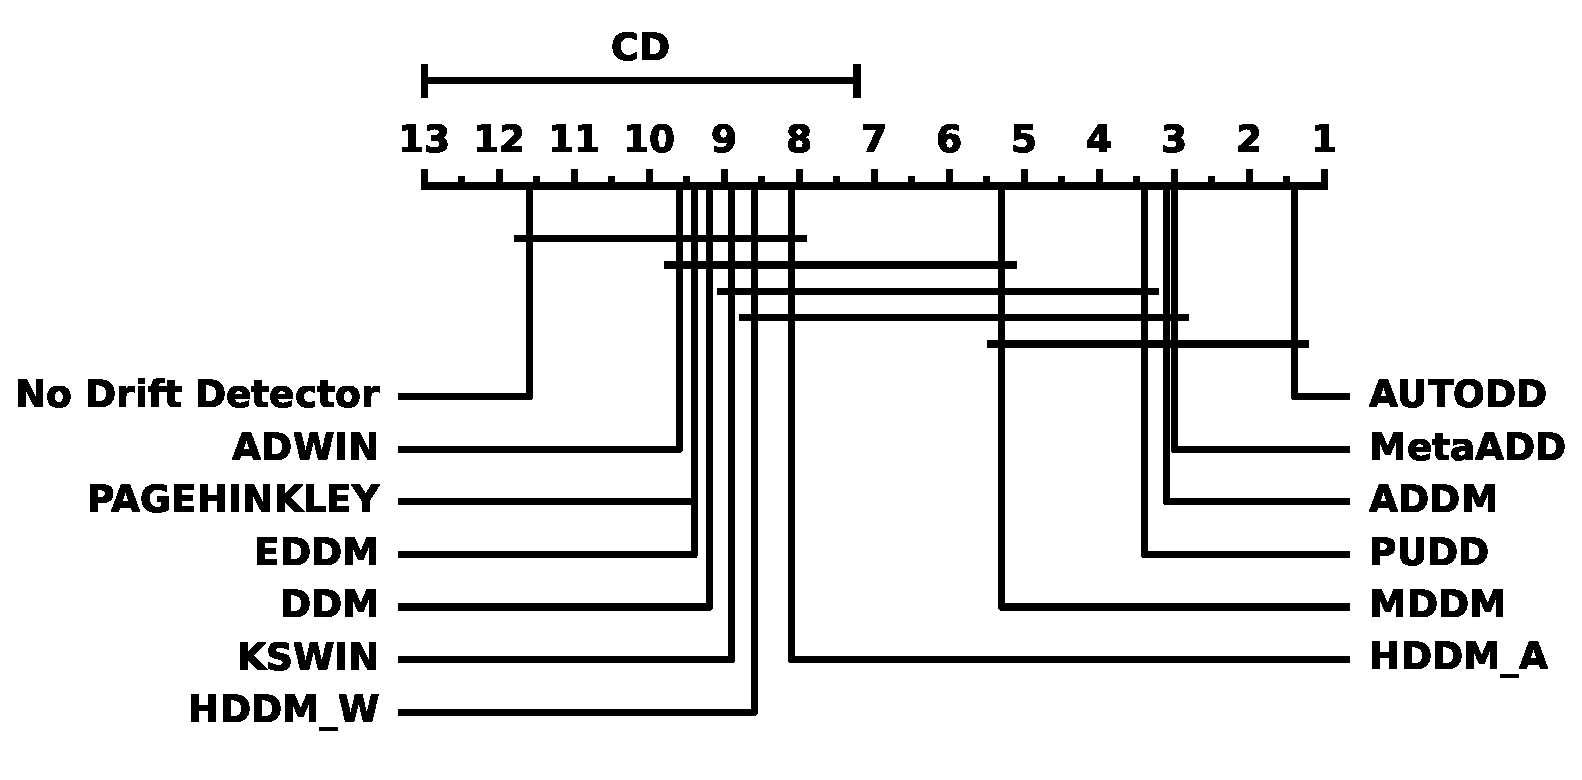
\includegraphics[width=\textwidth]{cd/cd_diagram_gaussiannb.pdf}\\[2pt]
  {\small\bfseries GaussianNB}
\end{minipage}\hfill
\begin{minipage}[t]{0.49\textwidth}
  \centering
  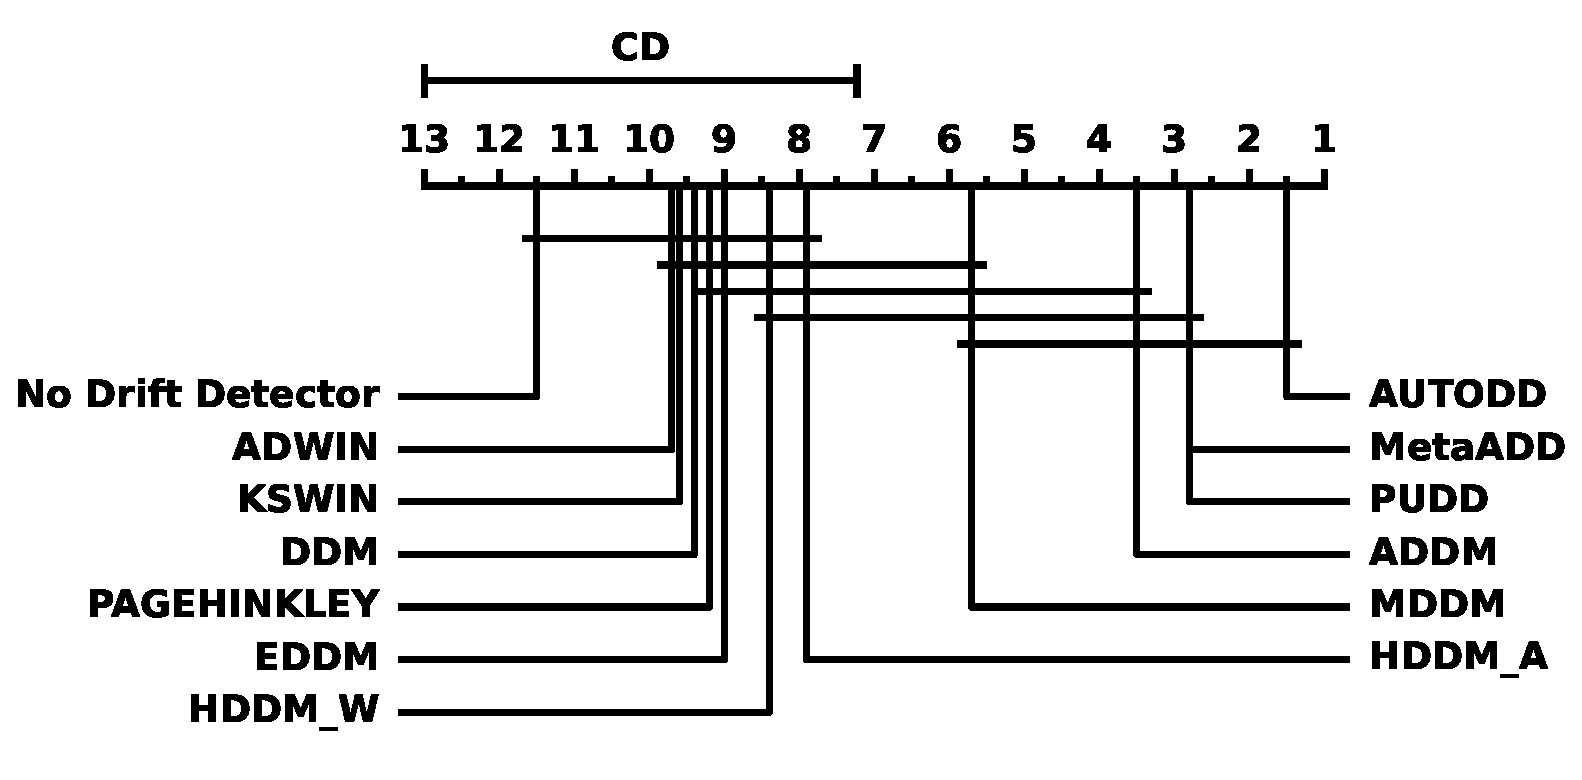
\includegraphics[width=\textwidth]{cd/cd_diagram_hat.pdf}\\[2pt]
  {\small\bfseries HAT}
\end{minipage}\par}
\end{block}}

\begin{block}{Ablation Study}
{\centering
\begin{tabular}{lcc}
\toprule
\textbf{Variant} & \textbf{Acc.} & \textbf{$\Delta$}\\
\midrule
Full AutoDD             & \textbf{80.5\%} & --\\
w/o Thompson (Level 2)  & 75.3\% & $-5.2$\\
w/o Temporal            & 74.2\% & $-6.3$\\
w/o Stationarity        & 73.5\% & $-7.0$\\
w/o Statistical         & 71.2\% & $-9.3$\\
w/o LinUCB (Level 1)    & 62.5\% & \textbf{\color{accent}$-18.0$}\\
\bottomrule
\end{tabular}\par}
\vskip10pt
Matching the detector to the stream is the primary driver. Configuration search and all
three meta-feature families add smaller, complementary gains, and AutoDD stays
in the fast, low-memory quadrant against every comparator.
\end{block}


\begin{block}{Conclusion and Future Work}
The drift detector no longer has to be chosen by hand. A contextual bandit
learns it online from a reward that needs no drift labels, and AutoDD attains
the best average rank on ten benchmarks under both base learners at competitive
computational cost.
\vskip8pt
\textbf{Future work.} Learning the window size $w$ in an outer adaptive loop,
replacing the accuracy-based proxy with a label-free reward, and granting
baselines an equivalent tuning budget so that the benefit of selection is
separated from the benefit of tuning.
\end{block}


\end{column}
\end{columns}
\paperidstamp

\end{frame}
\end{document}
